\doublespacing % Do not change - required

\chapter{Experimental Result and Discussion}
\label{ch4}

%%%%%%%%%%%%%%%%%%%%%%%%%%%%%%%%%%%%%%%
% IMPORTANT
\begin{spacing}{1} %THESE FOUR
\minitoc % LINES MUST APPEAR IN
\end{spacing} % EVERY
\thesisspacing % CHAPTER
% COPY THEM IN ANY NEW CHAPTER
%%%%%%%%%%%%%%%%%%%%%%%%%%%%%%%%%%%%%%%

\section{Cross-Method Quality Retention}
Model quality was compared using assistant-response perplexity under the
common UltraChat-200k \texttt{test\_sft} evaluation protocol. Lower
perplexity indicates better retention of the BF16 baseline behaviour.

\subsection{Perplexity Comparison}
Table~\ref{tab:cross-method-ppl} compares the perplexity obtained by the
principal quantization configurations.

\begin{table}[htbp]
\centering
\caption{Perplexity comparison across the evaluated quantization
configurations.}
\label{tab:cross-method-ppl}

\begin{spacing}{1}
\small
\renewcommand{\arraystretch}{1.20}

\begin{tabularx}{0.82\textwidth}{
@{}
>{\raggedright\arraybackslash}X
>{\centering\arraybackslash}p{0.22\textwidth}
@{}
}
\toprule
\textbf{Configuration} &
\textbf{Perplexity $\downarrow$} \\
\midrule

BF16 baseline             & 7.125503 \\
SmoothQuant W8A8KV16      & 7.159544 \\
NestQuant W4.25A16KV16    & 7.171211 \\
AWQ W4A16KV16             & 7.418013 \\
NestQuant W4.25A4KV4      & 7.421992 \\
Project-specific W4A8     & 7.488315 \\

\bottomrule
\end{tabularx}
\end{spacing}
\end{table}

It can be seen that SmoothQuant achieved the lowest perplexity among the quantized
configurations, followed closely by NestQuant W4.25A16KV16. The more
aggressive low-bit configurations produced larger deviations from the
BF16 baseline.

\subsection{Relative Quality Degradation}
Table~\ref{tab:relative-quality-degradation} summarises the relative
perplexity increase of each quantized configuration with respect to the
BF16 baseline.

\begin{table}[htbp]
\centering
\caption{Relative perplexity degradation with respect to the BF16 baseline.}
\label{tab:relative-quality-degradation}

\begin{spacing}{1}
\small
\renewcommand{\arraystretch}{1.18}

\begin{tabularx}{0.78\textwidth}{
@{}
>{\raggedright\arraybackslash}X
>{\centering\arraybackslash}p{0.24\textwidth}
@{}
}
\toprule
\textbf{Configuration} &
\textbf{Relative PPL Increase} \\
\midrule

SmoothQuant W8A8KV16   & +0.48\% \\
NestQuant W4.25A16KV16 & +0.64\% \\
AWQ W4A16KV16          & +4.11\% \\
NestQuant W4.25A4KV4   & +4.16\% \\
Project-specific W4A8  & +5.09\% \\

\bottomrule
\end{tabularx}
\end{spacing}
\end{table}

The percentage change provides a clearer indication of the relative
perplexity degradation. SmoothQuant and NestQuant W4.25A16KV16 exhibited
the most stable quality retention, with only minor increases relative to
the BF16 baseline.

\subsection{Discussion of Quality Retention}

The results show that lower numerical precision does not lead to a
uniform loss in model quality. SmoothQuant retained BF16 behaviour most
effectively, while NestQuant W4.25A16KV16 achieved similarly strong
quality retention at a substantially lower weight precision. More
aggressive quantization of weights and activations introduced a larger
quality penalty.

% ============================================================
\section{Compression and Memory Behaviour}

The memory comparison focuses on runtime model-tensor storage and peak
GPU memory. These two metrics show whether the reduced numerical
precision is translated into practical deployment-memory savings.

\subsection{Runtime Model-Tensor Storage}

Figure~\ref{fig:runtime-model-storage} shows the runtime
model-tensor storage of the evaluated implementations.

\begin{figure}[htbp]
    \centering
    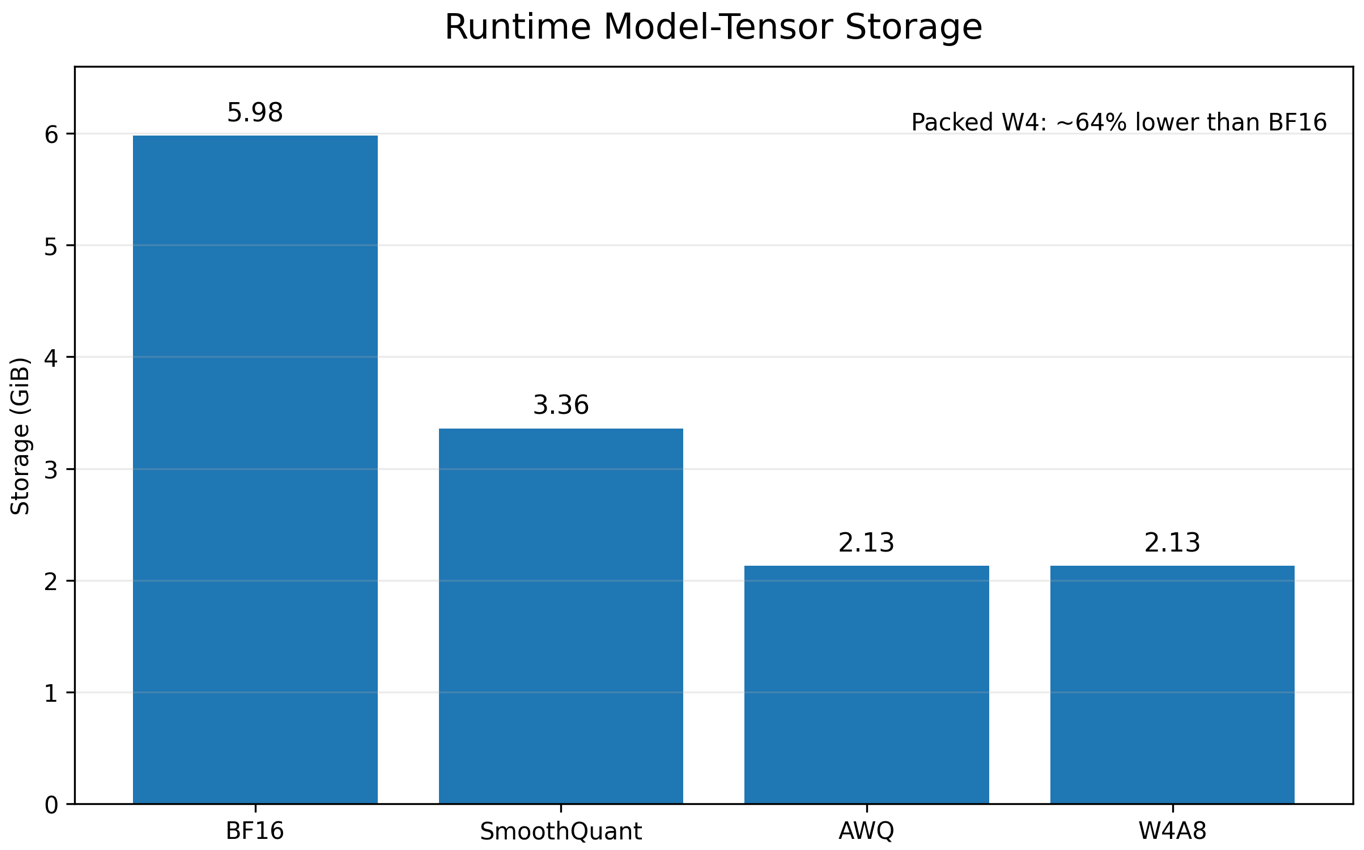
\includegraphics[width=0.72\textwidth]{imgs/runtime-model-tensor-storage.png}
    \caption{Runtime model-tensor storage across the evaluated configurations.}
    \label{fig:runtime-model-storage}
\end{figure}

BF16 required 5.98~GiB, SmoothQuant required 3.36~GiB, and both AWQ
and W4A8 required 2.13~GiB. Thus, the packed W4 configurations achieved
the lowest runtime model-tensor storage, reducing it by about 64\%
relative to BF16.

\subsection{Peak GPU Memory}

Figure~\ref{fig:peak-gpu-memory} compares the peak GPU memory required
by the evaluated implementations.

\begin{figure}[htbp]
    \centering
    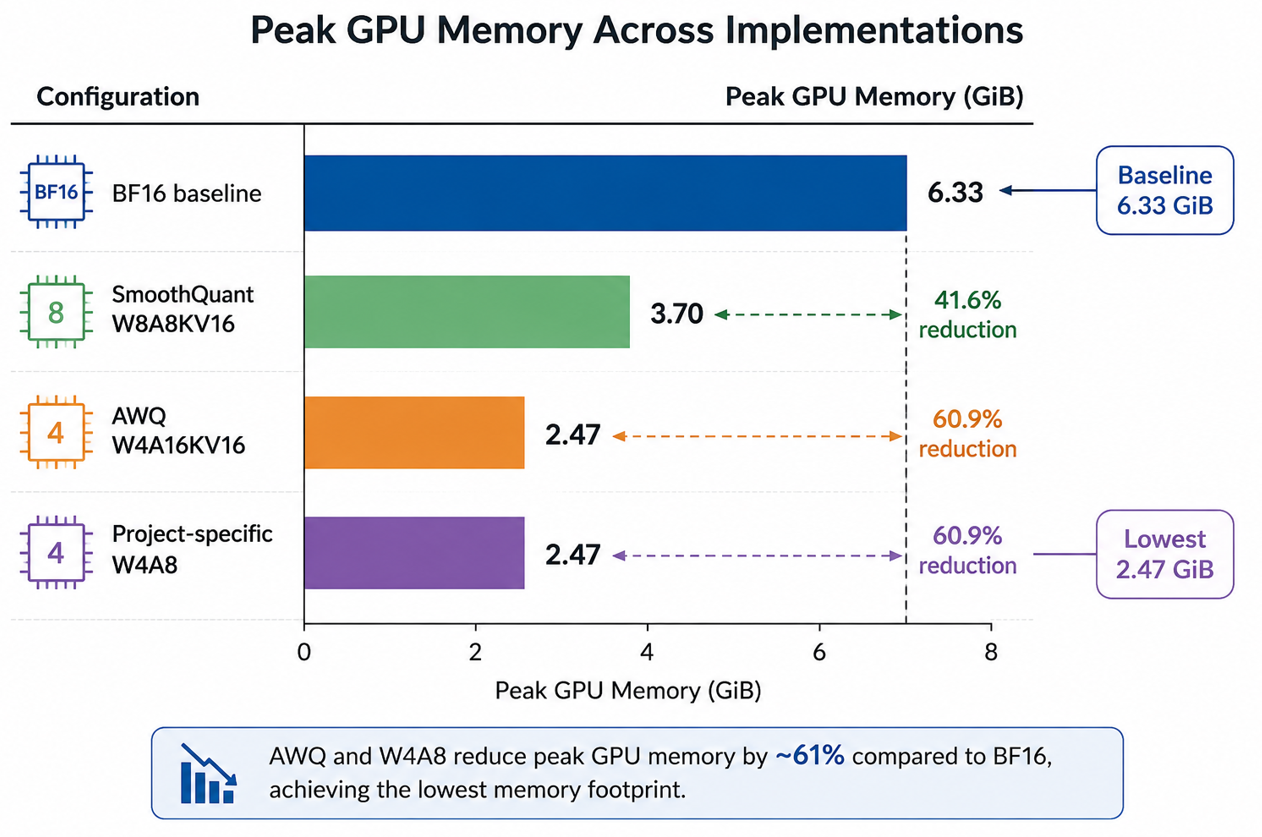
\includegraphics[width=0.72\textwidth]
    {imgs/peak-gpu-memory.png}
    \caption{Peak GPU memory across the evaluated configurations.}
    \label{fig:peak-gpu-memory}
\end{figure}

BF16 required 6.33~GiB of peak GPU memory, while SmoothQuant reduced
this to 3.70~GiB. AWQ and the project-specific W4A8 pipeline both
required 2.47~GiB, corresponding to a reduction of approximately
61\% relative to BF16.

\subsection{Discussion of Compression Efficiency}
The memory results show a clear relationship between weight precision
and compression efficiency. AWQ and the project-specific W4A8 pipeline
achieved the lowest runtime model storage and peak GPU memory, while
SmoothQuant occupied an intermediate position between the W4
configurations and the BF16 baseline.

The nearly identical memory footprints of AWQ and W4A8 indicate that
the packed 4-bit weight representation is the dominant source of memory
reduction in these configurations. Extending the W4A8 pipeline to
dynamic INT8 activations did not materially reduce the persistent model
footprint further. Therefore, practical compression depends not only on
nominal precision, but also on which tensor classes are quantized and
whether the low-bit representation remains packed during runtime.


% ============================================================
\section{NestQuant Quantization-Scope Ablation}
The NestQuant ablation evaluates how extending quantization from weights
to the KV cache and activations affects model quality. The
W4.25A16KV16 configuration is used as the internal reference.

\subsection{KV-Cache Quantization}
Reducing the KV-cache precision from KV16 to KV4 increased perplexity
from 7.171211 to 7.224471, corresponding to a relative increase of only
\(0.743\%\).

\begin{equation}
\mathrm{W4.25A16KV16}
\rightarrow
\mathrm{W4.25A16KV4}
:
\quad
\Delta \mathrm{PPL}=+0.743\%.
\end{equation}

This indicates that KV-cache quantization produced only a small quality
penalty under the evaluated configuration.

\subsection{Activation Quantization}
Reducing activation precision from A16 to A4 increased perplexity from
7.171211 to 7.382130, giving a relative increase of \(2.941\%\).

\begin{equation}
\mathrm{W4.25A16KV16}
\rightarrow
\mathrm{W4.25A4KV16}
:
\quad
\Delta \mathrm{PPL}=+2.941\%.
\end{equation}

The degradation is substantially larger than that caused by KV4,
showing greater sensitivity to activation quantization.

\subsection{Combined Activation and KV-Cache Quantization}

Applying both A4 and KV4 produced a perplexity of 7.421992, corresponding
to a \(3.497\%\) increase relative to W4.25A16KV16.

\begin{equation}
\mathrm{W4.25A16KV16}
\rightarrow
\mathrm{W4.25A4KV4}
:
\quad
\Delta \mathrm{PPL}=+3.497\%.
\end{equation}

This configuration represents the broadest NestQuant quantization scope
evaluated in this study.

\subsection{Discussion of Quantization Sensitivity}
Table~\ref{tab:nestquant-sensitivity} compares the absolute and relative
perplexity changes introduced by extending the NestQuant quantization
scope from the W4.25A16KV16 reference configuration.

\begin{table}[htbp]
\centering
\caption{Absolute and relative perplexity degradation for NestQuant
quantization.}
\label{tab:nestquant-sensitivity}

\begin{spacing}{1}
\small
\renewcommand{\arraystretch}{1.18}

\begin{tabularx}{0.92\textwidth}{
@{}
>{\raggedright\arraybackslash}X
>{\centering\arraybackslash}p{0.16\textwidth}
>{\centering\arraybackslash}p{0.16\textwidth}
>{\centering\arraybackslash}p{0.16\textwidth}
@{}
}
\toprule
\textbf{Quantization change} &
\textbf{PPL} &
\textbf{Absolute $\Delta$PPL} &
\textbf{Relative $\Delta$PPL} \\
\midrule

W4.25A16KV16
&
7.171211
&
0.000000
&
0.000\% \\

KV16 $\rightarrow$ KV4
&
7.224471
&
+0.053260
&
+0.743\% \\

A16 $\rightarrow$ A4
&
7.382130
&
+0.210919
&
+2.941\% \\

A16KV16 $\rightarrow$ A4KV4
&
7.421992
&
+0.250781
&
+3.497\% \\

\bottomrule
\end{tabularx}
\end{spacing}
\end{table}

Both the absolute and percentage changes show that activation
quantization is substantially more quality-sensitive than KV-cache
quantization. The relative A4 penalty is approximately four times the
KV4 penalty, while the combined A4+KV4 configuration produces the
largest overall degradation.


\section{Packed NestQuant Deployment Performance}

This section evaluate separate packed W4.25A16KV16 implementation to determine
whether the low-bit representation translated into practical deployment
benefits in storage, GPU memory and runtime performance.

\subsection{Packed Representation and Storage}

To verify whether the low-bit NestQuant configuration translated into a
genuinely smaller deployable artefact, the serialized checkpoint size
was compared between the floating-point reference and the packed
NestQuant implementation. As shown in Figure~\ref{fig:packed-checkpoint-size},

\begin{figure}[htbp]
    \centering
    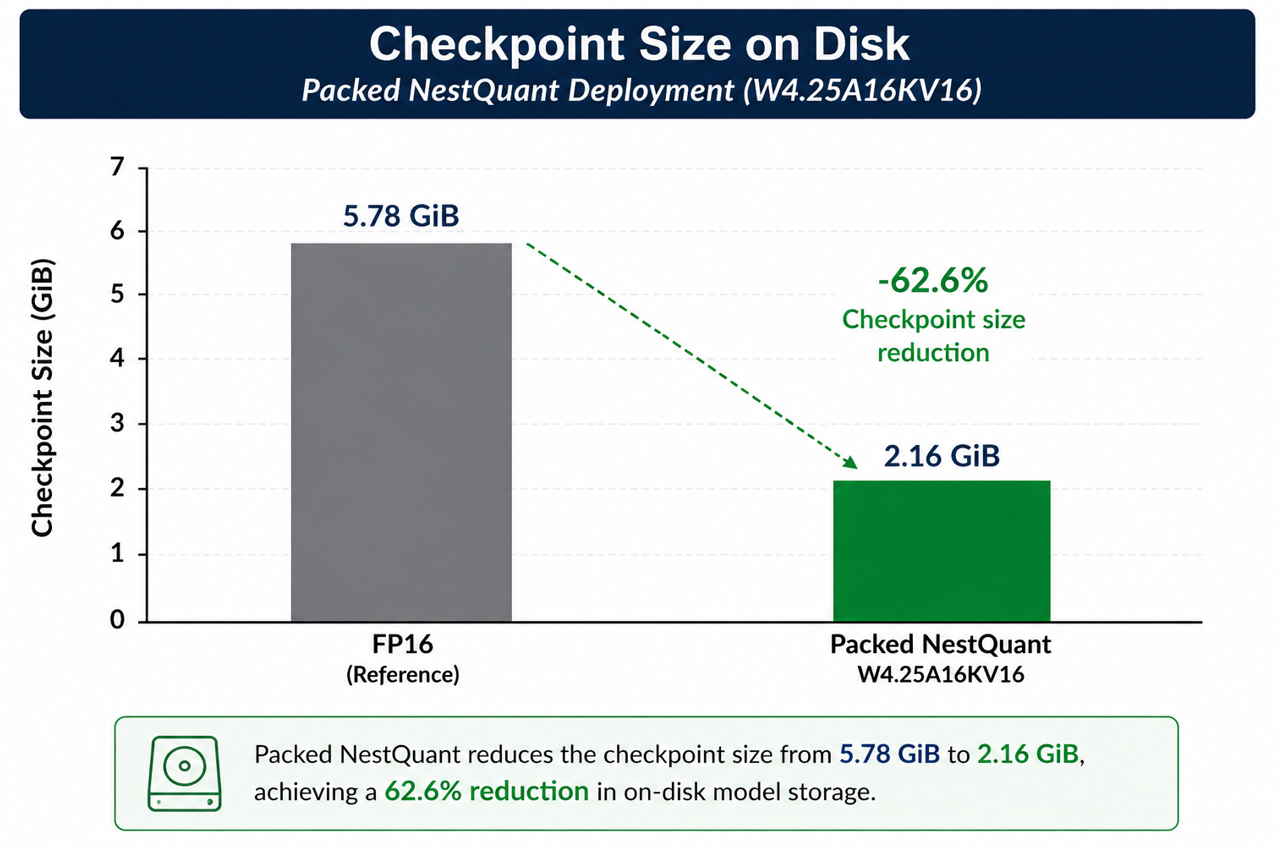
\includegraphics[width=0.58\textwidth]{imgs/packed-nestquant-checkpoint-size.png}
    \caption{Checkpoint size for packed NestQuant W4.25A16KV16 deployment path. }
    \label{fig:packed-checkpoint-size}
\end{figure}

the FP16 reference required 5.78~GiB, whereas the packed
NestQuant W4.25A16KV16 representation required only 2.16~GiB.
This corresponds to a checkpoint-size reduction of 62.6\%.

It confirms that the structured W4.25 representation was
successfully translated into a substantially smaller physical model
artefact rather than remaining only a nominal low-bit configuration.

\subsection{GPU-Memory Reduction}

Figure~\ref{fig:packed-nestquant-peak-gpu} compares the peak GPU memory
required by the FP16 baseline and the packed NestQuant deployment path.
Peak GPU memory decreased from 6.01~GiB for FP16 to 2.84~GiB for packed
NestQuant W4.25A16KV16, corresponding to a 52.7\% reduction.

So the packed deployment path substantially lowers
runtime memory demand while maintaining strong quality retention, making
it more practical for memory-constrained LLM deployment.

\begin{figure}[htbp]
    \centering
    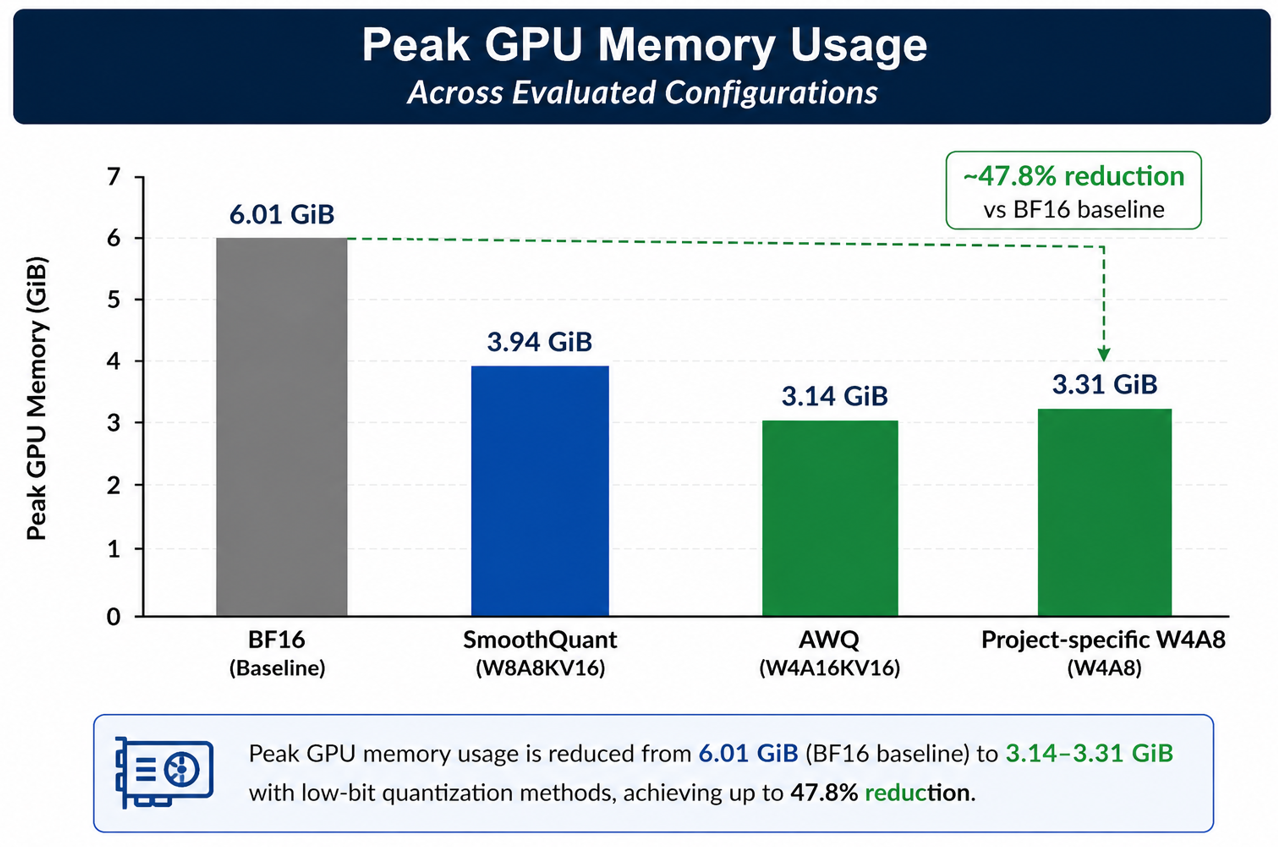
\includegraphics[width=0.62\textwidth]{imgs/packed_nestquant_peak_gpu_memory.png}
    \caption{Peak GPU memory comparison between the FP16 baseline and the packed
    NestQuant W4.25A16KV16 deployment path. Packed NestQuant reduces peak GPU
    memory from 6.01~GiB to 2.84~GiB, a reduction of 52.7\%.}
    \label{fig:packed-nestquant-peak-gpu}
\end{figure}

\subsection{Discussion of Deployment Behaviour}
The packed NestQuant W4.25A16KV16 representation provides clear
deployment advantages by translating low-bit quantization into a
substantially smaller physical model footprint. In comparison to the
floating-point reference, checkpoint size was reduced by 62.6\%, and
peak GPU memory decreased by 52.7\%.

These results demonstrate the practical value of maintaining the
NestQuant representation in packed form rather than reconstructing a
dense high-precision weight matrix. The reduced storage and memory
requirements improve deployment efficiency and make the model more
suitable for memory-constrained hardware environments.







